\newpage
\section{Data Preparation}

According to seminal research by \cite{Reference1}, lorem ipsum dolor sit amet.  However, this result was already known in the 1990s \citep{Reference2,Reference3}.  % Note the use of \cite{} and \citep{}


\section{A Section that Contains Some Maths}

\lipsum  % Replace with your text
 
\begin{equation}
M = \frac{1}{T}\sum_{t=1}^{T} e(t) / \max_{t}[e(t)]
\label{eq:equation}
\end{equation}

\lipsum  % Replace with your text

This is shown in Equation \ref{eq:equation} and is repeated here $M = \frac{1}{T}\sum_{t=1}^{T} e(t) / \max_{t}[e(t)]$.


\section{A Section that Contains a Figure}

\lipsum  % Replace with your text

\begin{figure}[ht]
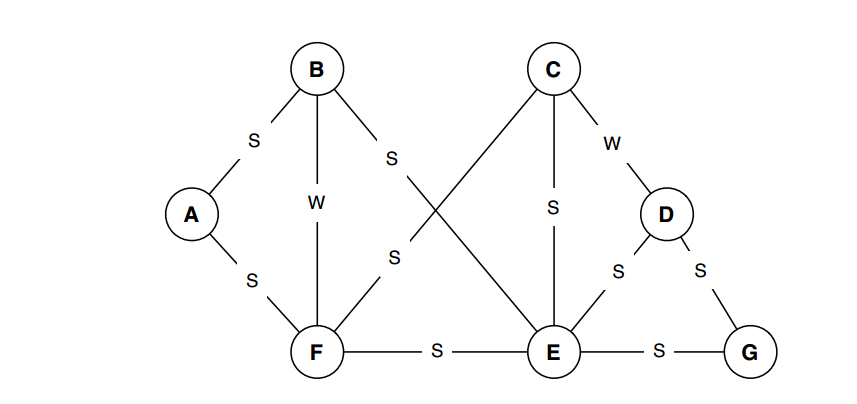
\includegraphics[width=15cm]{figures/figure1.png}
\caption{A simple figure in \LaTeX. Reproduced from http://tinyurl.com/nqtrlj5 with the permission of the copyright owner.}
\label{fig:graph}
\end{figure}

\lipsum  % Replace with your text

See Figure \ref{fig:graph}.


\section{A Section that Contains a Table}

\lipsum  % Replace with your text

\begin{table}[ht]
\center
\begin{tabular}{cc|c}
A & B & A XOR B\\
\hline
0 & 0 & 0\\
0 & 1 & 1\\
1 & 0 & 1\\
1 & 1 & 0\\
\end{tabular}
\caption{A simple table in \LaTeX.}
\label{tab:xor}
\end{table}

\lipsum  % Replace with your text

This is shown in Table \ref{tab:xor}.


\section{Summary}

\lipsum  % Replace with your text
